
與內存數據相比,CPU中的寄存器可以更快地對數據進行操作。處理器和內存的速度至少有一個數量級的差異,在沒有通過直接測量對性能進行驗證之前,不要對性能做出任何猜測或假設。不過這不意味著關於系統架構的先驗知識和基於這些知識的假設都沒用,假設可以用來指導實驗和設計正確的測試方法。我們將在本章中瞭解到,偶然嚐到的甜頭不會走太遠,甚至會誤入歧途。測試本身沒問題,但通常很難確定測量的是什麼,以及可以從結果中得出什麼結論。

測量內存訪問速度相當簡單,需要一些可以讀取內存和確定讀取時間的方法,像這樣:

\begin{lstlisting}[style=styleCXX]
volatile int* p = new int;
*p = 42;
for (auto _ : state) {
	benchmark::DoNotOptimize(*p);
}
delete p;
\end{lstlisting}

這個基準測試會運行和測試……一些東西。可以將一次迭代的時間報告為0納秒。這可能是不必要的編譯器優化結果。如果編譯器發現整個程序沒有可觀察行為,那麼確實可以將其優化為零。但是,針對這樣的事件採取了措施。讀取的內存是\texttt{volatile},訪問\texttt{volatile}內存會認為是一種可觀察行為,不能優化掉。相反,0納秒的結果在一定程度上是基準測試本身的缺陷,表明單次讀取的速度要快於1納秒。這裡測試到的內存速度與期望大相徑庭,我們不能從一個什麼都沒有的報告中得到任何東西,包括自己犯的錯誤。在修正基準測試方面,我們要做的就是在基準測試迭代中進行多次讀取,如下所示:

\begin{lstlisting}[style=styleCXX]
volatile int* p = new int;
*p = 42;
for (auto _ : state) {
	benchmark::DoNotOptimize(*p);
	… repeat 32 times …
	benchmark::DoNotOptimize(*p);
}
state.SetItemsProcessed(32*state.iterations());
delete p;
\end{lstlisting}

每次迭代執行32次讀取,可以從報告的迭代時間中計算出單個讀取的時間。讓谷歌基準庫為我們進行計算,並報告每秒讀取的次數。這可以通過在基準測試結束時,設置處理數量來實現。

基準測試在中等級別的CPU上,大約需要5納秒的迭代時間,從而確認單次讀取時間是總時間的1/32,遠低於1納秒(因此對每次迭代報告為0的猜測得到了驗證)。另一方面,這個值與我們對慢速內存的期望並不匹配,所以我們之前關於性能瓶頸的假設可能不正確,當然還可以測試內存速度之外的指標。

\subsubsubsection{4.3.1\hspace{0.2cm}內存架構}

為了理解如何正確地測試內存性能,必須更多地瞭解現代處理器的內存架構,內存系統最重要的特性是層級結構。CPU不直接訪問主存,而是通過緩存的層級結構進行:

%\hspace*{\fill} \\ %插入空行
\begin{center}
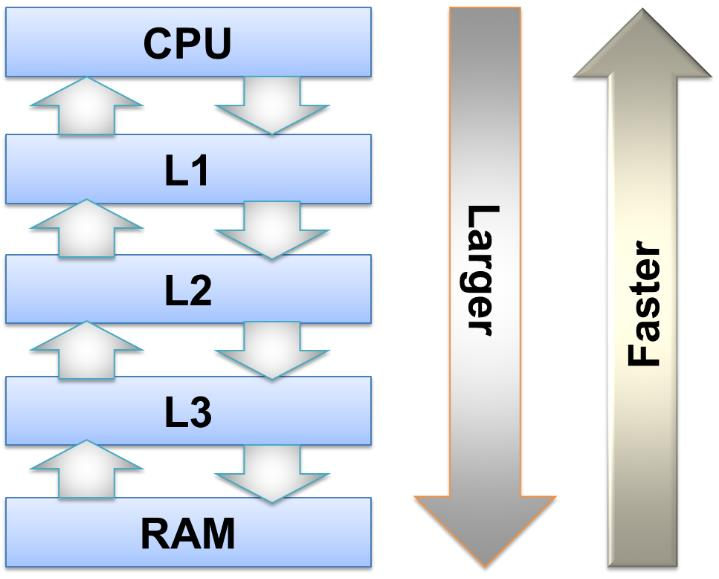
\includegraphics[width=0.5\textwidth]{content/1/chapter4/images/2.jpg}\\
圖4.2 - 內存層級結構圖
\end{center}

圖4.2中的\textbf{RAM}是主存儲器,即主板上的DRAM。系統說明書上說,這臺機器有這麼多G的內存,這就是DRAM的容量。可以看到,CPU並不直接訪問主內存,而是通過幾個層級結構的緩存訪問主內存。這些緩存也是內存電路,但它們位於CPU芯片內部,使用不同的技術來存儲數據,都是不同速度的SRAM。DRAM和SRAM的關鍵區別在於SRAM的訪問速度要快得多,但比DRAM的功耗要大得多。隨著我們在內存層級結構中越靠近CPU,內存訪問的速度就越快。level-1(\textbf{L1})緩存的訪問時間與CPU寄存器的訪問時間幾乎相同,但它功耗很大,以至於只能擁有幾千字節的內存空間,通常每個CPU核心有32KB的L1緩存。下一層,\textbf{L2}緩存更大但更慢,第三層(\textbf{L3})緩存更大但也更慢(通常在CPU的多核之間共享),層次結構的最後一層就是主存。

CPU第一次從主內存中讀取數據值,該值通過所有緩存級別傳播,其副本保留在緩存中。CPU再次讀取相同的值,不需要等待從主內存獲取值,因為相同值的副本已經存儲在L1緩存中。

讀取的數據需要適合L1緩存的長度,所有數據在第一次訪問時就會加載到緩存中,之後CPU只需要訪問L1緩存即可。如果訪問不在緩存中的值,並且緩存已滿,那麼必須從緩存中清除一些內容,為新值騰出空間。這個過程完全由硬件控制,它有一些方法,根據我們最近訪問的值(根據第一次近似,長時間沒有使用的數據可能很快就不再需要了),來確定我們最不可能再次需要哪個值。下一級緩存更大,但使用方式相同:只要數據在緩存中,就在那裡訪問它(離CPU越近越好)。否則,需要從下一級緩存取值,對於L3緩存來說,就是從主存取值,如果緩存已滿,一些其他的數據塊必須從緩存中去除(也就是被緩存遺忘,不過原始數據仍在主存中)。

由於反覆讀取相同的值成千上萬次,初始讀取的時間基本上可以忽略,測試所得的平均讀取時間是L1緩存的讀取時間。L1緩存的速度確實非常快,所以如果測試數據是32KB,就不需要擔心內存的讀取的性能差。不過,還是需要了解如何正確地測量內存性能,這樣才能得出相應的結論。

\subsubsubsection{4.3.2\hspace{0.2cm}測試內存和緩存的速度}

已經理解了內存速度比一次讀取的時間要複雜得多,現在可以設計一個更合適的基準測試。可以預期緩存大小會對結果有影響,因此必須訪問不同大小的數據,從幾千字節(適合32KB的L1緩存)到幾十兆字節或更多(L3緩存大小不同,但通常在8MB到12MB之間)。由於對於大數據量測試,內存系統將從緩存中清除舊數據,所以可以預期性能取決於預測的情況,或者說取決於訪問模式。所謂的訪問,例如複製一個內存範圍,可能會以非常不同方式結束,而不是以隨機的順序訪問相同的範圍。最後,結果可能取決於內存訪問的粒度,訪問64位的值比訪問單個字符,哪個快?

連續讀取大數組的基準測試:

\hspace*{\fill} \\ %插入空行
\noindent
\textbf{01c\_cache\_sequential\_read.C}
\begin{lstlisting}[style=styleCXX]
template <class Word>
void BM_read_seq(benchmark::State& state) {
	const size_t size = state.range(0);
	void* memory = ::malloc(size);
	void* const end = static_cast<char*>(memory) + size;
	volatile Word* const p0 = static_cast<Word*>(memory);
	Word* const p1 = static_cast<Word*>(end);
	for (auto _ : state) {
		for (volatile Word* p = p0; p != p1; ) {
			REPEAT(benchmark::DoNotOptimize(*p++);)
		}
		benchmark::ClobberMemory();
	}
	::free(memory);
	state.SetBytesProcessed(size*state.iterations());
	state.SetItemsProcessed((p1 - p0)*state.iterations());
}
\end{lstlisting}

編寫的基準測試與之前非常類似,只是在主循環中做了一行修改:

\hspace*{\fill} \\ %插入空行
\noindent
\textbf{01d\_cache\_sequential\_write.C}
\begin{lstlisting}[style=styleCXX]
Word fill = {}; // Default-constructed
for (auto _ : state) {
	for (volatile Word* p = p0; p != p1; ) {
		REPEAT(benchmark::DoNotOptimize(*p++ = fill);)
	}
	benchmark::ClobberMemory();
}
\end{lstlisting}

寫入數組的值並不重要。如果認為0有點特殊,那麼可以用其他值初始化\texttt{fill}。

使用\texttt{REPEAT}宏來避免多次手動複製代碼。我們仍然希望每次迭代執行幾次內存讀取。當開始報告每秒讀取的數量時,避免每次迭代0納秒的報告就不重要了,但是對於這樣成本非常低的迭代來說,循環本身的開銷並不小,所以最好手動展開這個循環。\texttt{REPEAT}宏將循環展開32次:

\begin{lstlisting}[style=styleCXX]
#define REPEAT2(x) x x
#define REPEAT4(x) REPEAT2(x) REPEAT2(x)
#define REPEAT8(x) REPEAT4(x) REPEAT4(x)
#define REPEAT16(x) REPEAT8(x) REPEAT8(x)
#define REPEAT32(x) REPEAT16(x) REPEAT16(x)
#define REPEAT(x) REPEAT32(x)
\end{lstlisting}

當然,必須確保請求的內存大小足夠容納32個\texttt{Word}類型的值,並且數組的總大小能被32整除,這對基準測試代碼來說都不是什麼限制。

說到\texttt{Word}類型,這是第一次使用\texttt{TEMPLATE}基準測試。它用於在不復制代碼的情況下為幾種類型生成基準測試:

\begin{lstlisting}[style=styleCXX]
#define ARGS ->RangeMultiplier(2)->Range(1<<10, 1<<30)
BENCHMARK_TEMPLATE1(BM_read_seq, unsigned int) ARGS;
BENCHMARK_TEMPLATE1(BM_read_seq, unsigned long) ARGS;
\end{lstlisting}

如果CPU支持,可以在更大的塊中讀寫數據,例如:在x86 CPU上使用SSE和AVX指令一次移動16或32個字節。在GCC或Clang中,對於這些較大的類型,有一些頭文件:

\begin{lstlisting}[style=styleCXX]
#include <emmintrin.h>
#include <immintrin.h>
…
BENCHMARK_TEMPLATE1(BM_read_seq, __m128i) ARGS;
BENCHMARK_TEMPLATE1(BM_read_seq, __m256i) ARGS;
\end{lstlisting}

\texttt{\_\_m128i}和\texttt{\_\_m256i}類型沒內置在語言中(至少不是C/C++),但C++可以很容易地聲明新類型。這些是值類型類(表示單個值的類),有一組定義好的算術操作(加法和乘法),編譯器使用適當的SIMD指令來實現這些操作。

前面的基準測試依次訪問內存範圍,從開始到結束。內存的大小隨基準參數的指定而變化(在本例中,從1KB到1GB,每次增加一倍)。當複製一定範圍的內存時,基準測試會從頭再做一次,直到積累足夠的量。

當以隨機順序測量訪問內存速度,必須小心。天真的對代碼進行基準測試看起來可能會像這樣:

\begin{lstlisting}[style=styleCXX]
benchmark::DoNotOptimize(p[rand() % size]);
\end{lstlisting}

但此基準測試了調用\texttt{rand()}函數所需的時間,計算開銷比讀取單個整數要大得多,因此可能永遠不會注意到後者的開銷。取模運算符\texttt{\%}比單個讀或寫開銷大得多。獲得精確結果的唯一方法是預先計算隨機索引,並將它們存儲在另一個數組中。當然,現在正在同時讀取索引值和索引數據,所以測量的開銷是兩次讀取(或一次讀取和一次寫入)。

隨機寫入內存的代碼如下所示:

\hspace*{\fill} \\ %插入空行
\noindent
\textbf{01b\_cache\_random\_write.C}
\begin{lstlisting}[style=styleCXX]
const size_t N = size/sizeof(Word);
std::vector<int> v_index(N);
for (size_t i = 0; i < N; ++i) v_index[i] = i;
std::random_shuffle(v_index.begin(), v_index.end());
int* const index = v_index.data();
int* const i1 = index + N;
Word fill; memset(&fill, 0x0f, sizeof(fill));
for (auto _ : state) {
	for (const int* ind = index; ind < i1; ) {
		REPEAT(*(p0 + *ind++) = fill;)
	}
	benchmark::ClobberMemory();
}
\end{lstlisting}

使用STL算法\texttt{random\_shuffle}來產生隨機的索引順序(可以用隨機數代替,這並不完全相同,因為一些指數可能出現過不止一次,而另一些則從未出現過,但這不會對結果產生太大影響)。處理的值實際上不重要,編寫任何數字都需要相同的時間,但是編譯器有時可以進行優化,如果它能夠發現代碼出現了大量的零,那麼最好避免這種情況。另外,較長的AVX類型不能用整數初始化,因此可以使用\texttt{memset()}寫入值。

當然,讀取的基準測試代碼非常相似,只是內部循環進行了修改:

\begin{lstlisting}[style=styleCXX]
REPEAT(benchmark::DoNotOptimize(*(p0 + *ind++));)
\end{lstlisting}

基準測試代碼主要用於測量內存訪問的開銷,而對索引的運算不可避免,但是加法最多隻需要一個時鐘週期(CPU可以同時做幾個),所以數學運算不會成為瓶頸(而且,訪問數組內存的程序都必須做相同的計算,因此這就是實際中的訪問速度)。來看看結果吧!




























